\documentclass[11pt,a4paper]{article}
\usepackage{ls}
\usepackage[english]{babel}

\title{Business Modelling Basics, ISO 9000 and CMMI}  

\author{Hans-Gert Gr\"abe}

\date{25 April 2021}

\begin{document}
\maketitle

\section{Dimensions of a Systemic Approach}

The subject of our seminar are aspects of systematic management of planned
cooperative action, especially in the form of entrepreneurial organisations.

We had approached the topic in the last seminar and identified as a meaningful
starting point the concept of a \textbf{system} 
\begin{itemize}[noitemsep]
\item as a \emph{whole} composed of \emph{parts} 
\item with a \emph{specific purpose} (a \emph{main useful function} -- MUF),
\item which results from the \emph{interaction} of the functionalities of the
  parts as an \emph{emergent function}.
\end{itemize}
Systems thus have a structural, a functional and an operational dimension.

The \textbf{structural dimension} (structural organisation) is especially
important for understanding the system as a white box (i.e. its
implementation).

The \textbf{functional dimension} is a specific, complexity-reducing form of
both the description and the real-world organisation of complex functional
processes (procedural organisation) using the principle of encapsulation,
which is also widespread in computer science.

Finally, in the \textbf{operational dimension}, the functions are linked with
the resources required for their functioning and thus functions are
transferred from a pure potentiality into a (potential) reality.

Operationality means that not only the MUF of the system is constituted from
the functionalities of the parts in the way described in the procedural
organisation, but that the system also creates the operational conditions for
the functioning of its parts.

In this sense, the \emph{world of technical systems} (lecture) is itself again
a system, although structural and procedural organisation at the system level
are largely unknown in terms of description. This system is a "self-moving
automaton" in the sense of Marx's statement 
\begin{quote}
  [\ldots] set in motion by an automaton, a moving power that moves itself;
  this automaton consists of numerous mechanical and intellectual organs, so
  that the workers themselves are cast merely as its conscious linkages." (MEW
  42, ch. 13)
\end{quote}
This system functions "by itself" because the parts mutually produce their
respective necessary operational throughput conditions. That system has
\textbf{no external standpoint of planning} for this, but it does draw on
external material and energetic resources.

\section{Shchedrovitsky \cite{MSM} on Organisations}

What is an organisation? Shchedrovitsky \cite[p. 30 ff]{MSM} distinguishes
three dimensions of that notion
\begin{itemize}[noitemsep]
\item Organisational work
\item Organisation as the result and means of organisational work
\item Organisation as a form of life of the collective
\end{itemize}

\paragraph{Organisational work.}
When we organise we collect something. Let us take a look at design. We need
some structural elements, so there is a designer with a set of elements. We
must collect these elements in a particular way, and we must establish some
kind of connection and relations between them. When we are doing this sort of
work we must impose some organisational form on these elements. [\ldots]

And when we have done such work on the integration of the elements and the
establishment between them of certain relations and connections, we stop this
work, and then the whole, which we have organised, can begin to operate
according to its laws. But its action according to its laws no longer belongs
to organisational work.

Organisers deal with a particular set of elements, collect elements of a
certain type and form in particular quantities, combine them and set certain
relations and connections between them. When they have done this and have thus
created the structure of the organisation – and the structure is defined by
the location of the elements and the type of connections and relations – they
recede into the background, and this thing either remains dead or begins to
operate according to its laws.

\paragraph{Organisation as the result and means of organisational work.}
Organisation as the result of organisational work can be regarded as both an
\textbf{artificial entity} and as \textbf{naturally living thing}.

Who takes an artificial view of organisations? Organisers themselves. And
those who design and create organisations always looks at them as their own
creations.  The organiser makes it, and in this sense organisations can be of
any kind depending on the goals and objectives of the organiser. The main
question is: why does the organiser create a particular organisation?
[\ldots]

The organisation acts here as an \textbf{artificial entity}. It has a purpose
and can be considered, as can any structure, in terms of the functions that
it, the organisation, must provide. So we are talking about the functions of
the organisation, about the purpose of the organisation.  These are all
characteristics that are seen from an artificial point of view.

As a tool, as a means, \textbf{as an artificial entity, the organisation does
  not and cannot have goals}. Organisers can have goals. But for their goals,
in relation to their goals, the organisations they create are a means, a means
for them to achieve their goals.

\paragraph{Organisation as a form of life of the collective.}
The organisation has been created. And the organiser – a pure organiser, not a
manager – has gone. The organisation has been created, and it has begun to
live its own life. And then it turns out that, from a natural point of view,
other goals may appear in this organisation – the goals of the collective,
which was organised. Generally, something quite different begins, inasmuch as
this \textbf{organisation begins to live its own life}. Then we [\ldots] must
seek forms, methods, laws of the life of the groups and the collectives within
organisations.

When the organisation is seen from a natural viewpoint, it is not yet the
means, but the \textbf{form}, the \textbf{condition} of the life of the
collective (the people) who work in it.

And it is even possible to see the organisation in the same way as we see the
sunrise and sunset: the people working in it completely forget that the
organisation was created by some other person to resolve particular
objectives, achieve particular goals, for a particular purpose. It, this
organisation, will be perceived by them like the movement of the heavenly
bodies, as a natural condition of life.

\section{Shchedrovitsky \cite{MSM} on Management and Leadership\\ in
  Organisations} 

\paragraph{Management.}
[\ldots] Now a more complex case – a car. Here stands the car, you have not
yet pressed the accelerator – can you manage it? You cannot. And when does it
become possible to manage the car? When it has started moving.

\textbf{Management is only possible in relation to objects that have
  self-propulsion.}

Imagine a situation when you can control the flight of a chair. Imagine
yourself in a brawl from The Three Musketeers: someone throws a chair, and
instead of defending yourself from it, you send it flying the other way. You
have performed a one-off, momentary act of management – you changed the
direction of the flight of the chair. In this sense, you performed
\textbf{management of this process}. But what were you managing? You were
managing the flight of the chair, but not the chair.

\paragraph{Leadership.}
Leadership is only possible within an organisation, within the framework of
special organisational connections. The essence of leadership is the
\textbf{setting of goals and objectives for other elements}. But in order for
you to set goals and objectives for other elements – in other words, people –
they have to reject their own goals and objectives and undertake to accept
your goals and objectives. And that is precisely what happens in the framework
of the organisation.

The organisation of people always happens like this. The person who
\textbf{occupies a certain position} gives up their own goals and objectives,
their own self-propulsion (by the fact of occupying that position), and is
obliged to move only in accordance with this position and with the goals and
objectives that will be assigned to them through the channels of the
organisation by higher authorities.

But since people are not always aware that they must surrender their own goals
and objectives in carrying out their duties, and in addition, because people
who have surrendered their own goals and objectives are usually not much
useful for anything, the reality is that they only reject them within certain
limits. Such is the game. They pretend that they are ready to give up some of
their goals and accept other people’s goals and objectives, and what they
really mean to do is another question. They may temporarily conceal their own
goals, but they may use the performance of their official tasks to achieve
their own goals.

\textbf{When self-propulsion begins, leadership either becomes impossible or
  can only be carried out within a very narrow range, and the need for
  management appears.} Leaders not only lead, but also need to manage, because
their subordinates do not always entirely surrender their own goals, their
self-propulsion. But when self-propulsion begins, it will not be possible to
lead them. We have to use a different technique – the technique of management.

\section{Systematic Management in Organisations}

The subject of \emph{systematic management} are socio-technical and especially
socio-economic systems. The latter consist of economic units (companies, the
state, ... -- shortly \textbf{organisations}) that are interconnected in a
market-like manner. The \emph{world of economic units} has a systemic
structure similar to the world of technical systems.

In the understanding developed above, \textbf{management} therefore means to
\emph{control} the processes taking place in the (living) organisation with
the \emph{goal} to implement the \emph{purposes} of the organisation in an
efficient way.

This is necessary to be operated on several spatio-temporal levels (micro and
macro processes), whereby short term goals and long term goals are in 
contradictory tension. Therefore, management is usually divided into several
relatively autonomous levels
\begin{itemize}[noitemsep]
\item Strategic management
\item Middle management
\item Operational management
\item Infrastructure management and support
\end{itemize}
which are themselves in systemic system-subsystem interrelations and thus in a
co-evolutio\-nary relationship which is best processed via a control loop
designed as a feedback loop.

\subsection{Systematic Management and ISO 9000}

Systematic management requires a descriptive approach to this control loop as
part of the organisation's process model, such as given in the modified
process model of ISO 9000:2008.
\begin{center}
  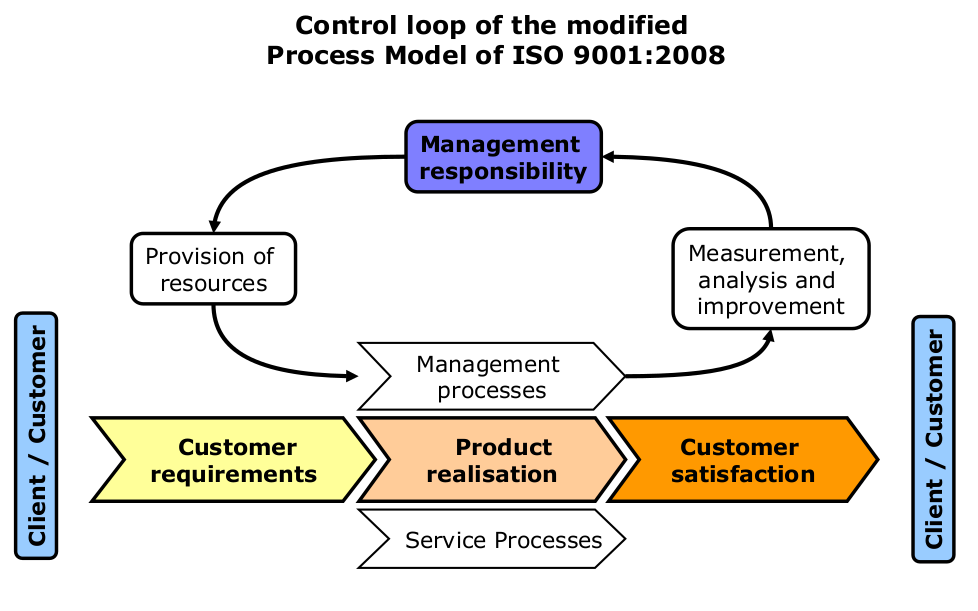
\includegraphics[width=.8\textwidth]{2.png}\\ \textbf{Fig. 1:} Control Loop
  in the Modified Process Model of ISO 9000
\end{center}
ISO 9000 is a set of general quality assurance standards to \textbf{assess}
the process quality of enterprises. It is a descriptive standard and not
directed towards improvement of process quality (although can be used for such
an improvement in combination with other tools).
\begin {itemize} [noitemsep]
\item It is mainly a European standard.
\item It is used mainly to assess the process quality of suppliers that
  demonstrate with a ISO 9000 certificate their ability to produce in a
  negotiated frame of time, costs and performance. 
\item Set of standards for the proof of process quality for the creation as of
  material so also of intangible products and services.
\item Framework with a lot of leeway for corporate strategy and concrete
  management goals.

  Minimum requirements for a QM system according to ISO 9000: complete,
  documented, known, verifiable, evolutionary
\end {itemize}
ISO 9000 contains minimum requirements for the structural and procedural
organization, so that quality is not a coincidence, but the result of a
controlled process.

Note that the process model shown in fig. 1 is a \emph{standard model} at a
higher language level (\textbf{meta-model}) than the respective process models
of the individual organisations, but unlike the process model of a real-world
organisation, it has no real-world instantiation. Such a phenomenon is well
known in computer science in connection with abstract classes.

Fig. 2 shows the relation between the ISO norm, quality management documents
and real-world process quality at three different levels within a company.  

\begin{center}
  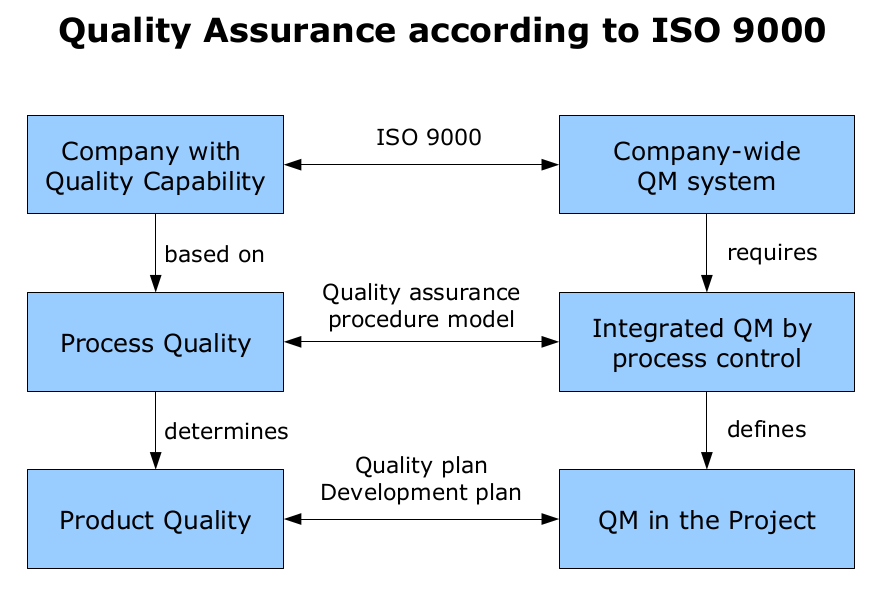
\includegraphics[width=.8\textwidth]{1.png}\\ \textbf{Fig. 2:} The relation
  between model, meta-model and meta-meta-model in quality assurance
\end{center}

\subsection{Managing Organisational Development and CMMI}

Management is only possible in the context of a clear understanding of the
structural and procedural organisation of the organisation.  In order to
capture this in descriptive terms, a \textbf{separation of functions and
  resources} is necessary. In particular, "human resources" are removed from
the description and replaced by the term \textbf{role}.

In this way, a \emph{functional decoupling from the resources} is achieved at
design time -- only at runtime this position must be connected "just in time"
with a qualified resource that was produced beyond the horizon of the concrete
planning processes.

Only with such a decoupling (and only at the level of such a decoupling) it is
possible as management to take an external standpoint on its own activities.
Only in this way is \textbf{structurally driven organisational development}
possible. There are other culturally driven approaches such as TQM, which will
be discussed separately (the Toyota model).

Systematic management through structurally driven organisational development
means above all the creation and improvement of conditions for the management
of well-structured processes.

CMMI (Capability Maturity Model and its predecessor CMM) is such a process
model for organisations such as software companies that are project-driven and
do not have a continuous production process. The model is a \textbf{maturity
  model} and supports such companies to introduce and improve a company-wide,
uniformly structured project management
\begin{itemize} [noitemsep]
\item from the structuring of individual projects into \emph{process
  activities and milestones}
\item through the definition of \emph{company-wide uniform or specifically
  adaptable process modules}
\item and the \emph{uniform quantitative measurement} of such building blocks
\item to the introduction of \emph{qualified error and change management}.
\end{itemize}
\begin{center}
  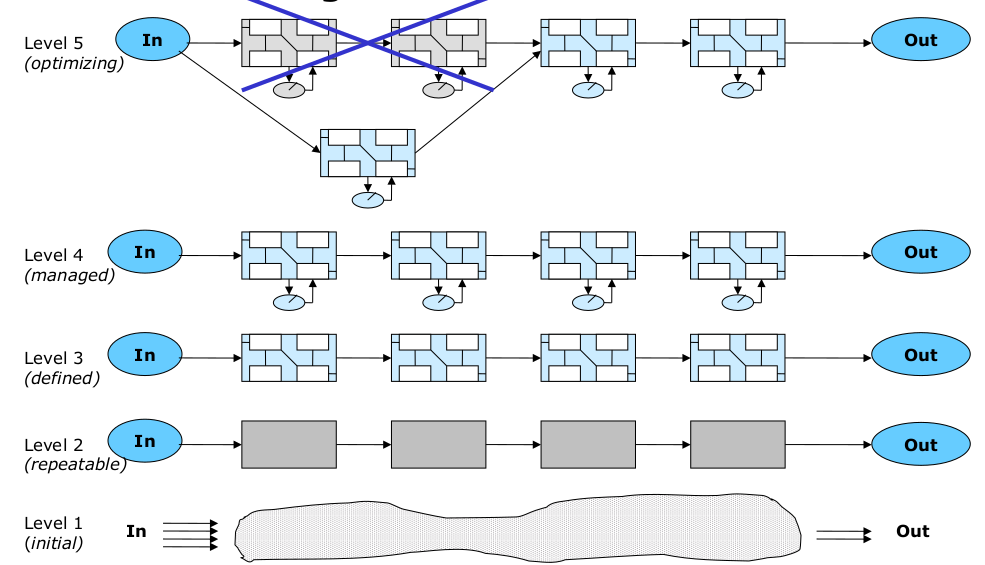
\includegraphics[width=.8\textwidth]{6.png}\\ \textbf{Fig. 3:} Increasing
  maturity of structured project management within CMM(I)
\end{center}
These four transitions are assigned five maturity levels. The transitions are
supported by concentrating on predefined \emph{key process areas} and
\emph{key practices}.

\subsection{Optional: CMMI in more detail}

\subsubsection{The Maturity Levels}

The five maturity levels according to which processes of an organization are
evaluated.

\paragraph {Initial Process}
\begin {itemize} [noitemsep]
\item Process exists only informally
\item Low adherence to deadlines and costs, high risk
\item Chaos, "heroism", fire-fighting operations
\end {itemize}

\paragraph {Repeatable Process (CMMI: Managed)}
\begin {itemize} [noitemsep]
\item There are defined and structured requirements for the process
\item "Learn from similar projects" (requirements management, project
  management and quality management)
\end {itemize}

\paragraph {Defined Process}
\begin {itemize} [noitemsep]
\item Procedures and individual process activities are clearly defined
\item The organization is in the learning focus
\item Process definition, training programs, team coordination
\end {itemize}

\paragraph {Managed Process (CMMI: Quantitatively Managed)}
\begin {itemize} [noitemsep]
\item Central control that systematically collects process measures
\item Process and product development are quantitatively analyzed and rated
\item Information is used as support for decision-making 
\end {itemize}

\paragraph {Optimizing Process}
\begin {itemize} [noitemsep]
\item "Self-dynamically optimizing process" 
\item Process measures are systematically used for dynamic process control and
  monitoring
\item Process change management
\item Technology change management
\end {itemize}

\subsubsection{Expectations}
The higher the level of maturity, 
\begin {itemize} [noitemsep]
\item the more precisely goals are achieved.
\item the less is the difference between the target and actual results.
  \begin {itemize} [noitemsep]
  \item Level 1 companies miss their deadlines at large. 
  \end {itemize}
\item The fluctuation range of the actual values around the target
  specifications is lower.
  \begin {itemize} [noitemsep]
  \item Similar projects are completed within a narrower time frame.
  \end {itemize}
\item Costs and development time decrease, productivity and quality increase.
  \begin {itemize} [noitemsep]
  \item Higher process efficiency, low rework rate.
  \end {itemize}
\item Expectations are more likely fulfilled in standard projects.
\item But: New techniques and applications are reducing the process capability
  due to higher variability.
\end {itemize}

\subsubsection{Determination of the Maturity Level according to CMM}

For each stage a number of \textbf {Key Process Areas} are defined in which an
organization of this level has to reposition itself implementing appropriate
given \textbf {Key Practices}.

\subsubsection*{Level 1: Initial Process}
\begin {itemize} [noitemsep]
\item No criteria and specifications
\item Project and quality management may or may not exist but are not 
  consistently applied.
\item Projects are managed at short notice, adaptively and reactively.
\end {itemize}

\subsubsection*{Level 2: Repeatable (CMMI: managed) Process}

\emph {Goal:} Introduction of a basic project monitoring and management,
planning and control.
  
\emph {Focus:} Leadership principles, structure and management of projects.

\emph {Key Process Areas and Key Practices:}
\begin {itemize} [noitemsep]
\item \textbf {Requirements management}
  \begin {itemize} [noitemsep]
  \item Establish a common understanding between customer and project team
    about the requirements.
  \end {itemize}
\item \textbf {Project planning, tracking and monitoring}
  \begin {itemize} [noitemsep]
  \item Transparent presentation of the development progress in order to be
    able to initiate correction measures at early stage.
  \end {itemize}
\item \textbf {Sub-order management}
  \begin {itemize} [noitemsep]
  \item Select, control and monitor qualified sub-suppliers.
  \end {itemize}
\item \textbf {Quality management} on process and product level, configuration
  management
  \begin {itemize} [noitemsep]
  \item Ensure integrity of the products throughout their entire life cycle.
  \end {itemize}
\end {itemize}

\emph{Result:}
\begin {itemize} [noitemsep]
\item Processes as a sequence of "black boxes" with milestones as checkpoints.
\item Stable project management.
\item Processes can be predicted within limits through constant monitoring.
\item Cross-project experience can be quantified.
\end {itemize}

\subsubsection*{Level 3: Defined Process}

\emph{Goal:} Definition and introduction of an organization-wide valid unified
software process; internal structure of the phases is defined and
understanding of roles is visible.

\emph {Prerequisite:} Projects are planned, managed and monitored (level 2) as
a sequence of processes according to uniform principles.

\emph {Focus:} Process descriptions.

\emph {Key Process Areas and Key Practices:} Focus on process organization
\begin {itemize} [noitemsep]
\item \textbf {Definition} of processes
  \begin {itemize} [noitemsep]
  \item Development and maintenance of a useful set of process values.
  \end {itemize}
\item \textbf {Training program}
  \begin {itemize} [noitemsep]
  \item An independent unit is responsible for employees' training.
  \end {itemize}
\item \textbf {Coordination} between project teams (exchange of experience)
\item \textbf {Integrated SW Management}
  \begin {itemize} [noitemsep]
  \item Development and management are integrated into one over the entire
    life cycle defined process.
  \item Standard processes can be tailored to projects.
  \end {itemize}
\item \textbf {SW Product engineering}
  \begin {itemize} [noitemsep]
  \item Process integrates all technical activities to ensure to produce
    correct, consistent products effectively and efficiently.
  \end {itemize}
\end {itemize}

CMMI further subdivides some of the main process areas
\begin {itemize} [noitemsep]
\item \textbf {Coordination}
  \begin {itemize} [noitemsep]
  \item Integrated team building
  \item Integrated sub-order management
  \item Decision analysis
  \item Integration organization infrastructure
  \end {itemize}
\item \textbf {Integrated SW Management}
  \begin {itemize} [noitemsep]
  \item Integrated project management
  \item Risk management
  \end {itemize}
\item \textbf {SW Product Engineering}
  \begin {itemize} [noitemsep]
  \item Requirements analysis
  \item Technical solution
  \item Product integration
  \item Verification
  \item Validation
  \end {itemize}
\end {itemize}

\emph{Result:} Improved, describable quality; institutionalised process
prototypes that are maintained and further developed.

\subsubsection*{Level 4: Managed (CMMI: Quantitatively Managed) Process}

\emph{Objective:} Quantitative measurement of the quality of products and the
productivity of processes through an organisation-wide metrics programme as an
objective basis for decision making.

\emph{Prerequisite:} Uniform understanding across the organisation about
projects and process models (level 3) and active project management (level 2).

\emph{Focus:} Process measurement.

\emph{Key Process Areas and Key Practices:}
\begin{itemize}[noitemsep]
\item \textbf{Quantitative process management}
  \begin{itemize}[noitemsep]
  \item Quantitatively control and monitor process performance.
  \end{itemize}
\item \textbf{Quantitative quality managament}
  \begin{itemize}[noitemsep]
  \item  Develop quantitative understanding of product quality.
  \end{itemize}
\end{itemize}

CMMI clarifies as follows:
\begin{itemize}[noitemsep]
\item Quantitative project management
\item Performance of organisational processes
\end{itemize}

\emph{Result:} Time, cost and quality become fairly predictable.

\subsubsection*{Level 5: Optimising Process}

\emph{Objective:} Introduction of a continuous and measurable process for
improvement of software development.

\emph{Prerequisite:} Quantitative monitoring information (level 4) and
application of innovative ideas and technologies.

\emph{Focus:} Process alignment.

\emph{Key Process Areas and Key Practices:}
\begin{itemize}[noitemsep]
\item \textbf{Error avoidance}
  \begin{itemize}[noitemsep]
  \item Identify and eliminate causes of errors.
  \end{itemize}
\textbf{Product innovation management}
  \begin{itemize}[noitemsep]
  \item Integration of new technological developments at product level.  
  \end{itemize}
\textbf{Process innovation management}
  \begin{itemize}[noitemsep]
  \item Identification of new, useful ideas and their orderly introduction.
  \end{itemize}
\end{itemize}
CMMI specified:
\begin{itemize}[noitemsep]
\item Organisation-wide introduction of innovations
\item Analysis of causes and elimination of errors
\end{itemize}


\begin{thebibliography}{xxx}
\bibitem{MSM} Victor B. Khristenko, Andrei G. Reus, Alexander P. Zinchenko et
  al. (2014). Methodological School of Management. Bloomsbury Publishing. ISBN
  978-1-4729-1029-5.
\end{thebibliography}

\end{document}

